\documentclass[tikz,border=8pt]{standalone}
\usepackage{amsmath}
\usetikzlibrary{arrows.meta,decorations.pathreplacing}
\begin{document}

% Asset ID: AS2DataPresentationTikZ-008
% Source: Comparing box plots evidence.
% Related lesson section: Exam Technique, Comparing Distributions.
% Purpose: Compare two box plots using location and spread.
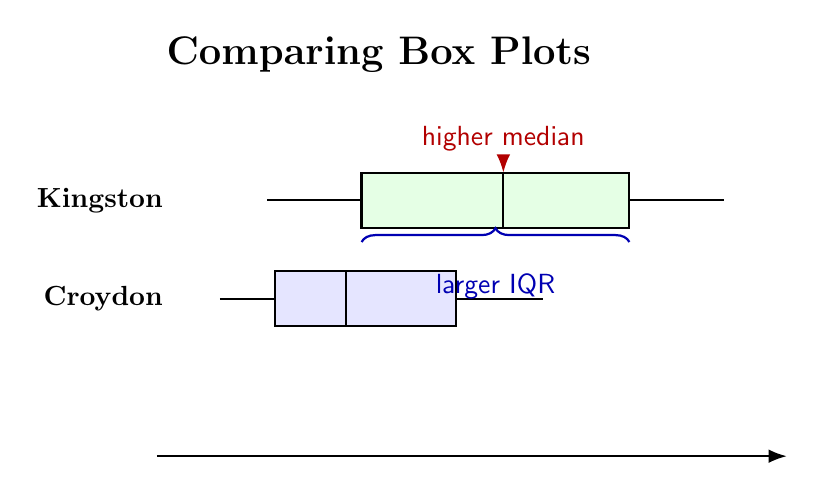
\begin{tikzpicture}[x=0.02cm,y=1cm,>=Latex,font=\sffamily]
\node[anchor=west,font=\bfseries\Large] at (380,5.1){Comparing Box Plots};
\draw[->,thick] (380,0)--(780,0);
\node[left,font=\bfseries] at (390,2.0){Croydon};
\draw[thick] (420,2)--(455,2); \draw[thick,fill=blue!10] (455,1.65) rectangle (570,2.35); \draw[thick] (500,1.65)--(500,2.35); \draw[thick] (570,2)--(625,2);
\node[left,font=\bfseries] at (390,3.25){Kingston};
\draw[thick] (450,3.25)--(510,3.25); \draw[thick,fill=green!10] (510,2.9) rectangle (680,3.6); \draw[thick] (600,2.9)--(600,3.6); \draw[thick] (680,3.25)--(740,3.25);
\draw[->,red!70!black,thick] (600,3.75)--(600,3.6); \node[above,red!70!black] at (600,3.75){higher median};
\draw[decorate,decoration={brace,amplitude=5pt},blue!70!black,thick] (510,2.72)--(680,2.72) node[midway,below=8pt]{larger IQR};
\end{tikzpicture}

\end{document}
